\documentclass[12pt, letterpaper]{article}
\usepackage{graphicx} % Required for inserting images
\usepackage{hyperref}
\usepackage{listings}
\usepackage{amssymb}
\usepackage{amsmath}
\usepackage[english]{babel}
\usepackage{amsfonts}
\usepackage{nicefrac, xfrac}
\usepackage[utf8]{inputenc}
\usepackage{mathtools}
\newcommand{\acc}{\\\hphantom{}\\}
\usepackage[dvipsnames]{xcolor}
\usepackage[titles]{tocloft} % Optional: Better control of the table of contents

\definecolor{light-gray}{gray}{0.95}
\newcommand{\code}[1]{\colorbox{light-gray}{\texttt{#1}}}
\newcommand{\codee}[1]{\colorbox{white}{\texttt{#1}}}
\usepackage[paper=a4paper,left=20mm,right=20mm,bottom=25mm,top=25mm]{geometry}
\renewcommand{\labelenumii}{\arabic{enumi}.\arabic{enumii}}
\renewcommand{\labelenumiii}{\arabic{enumi}.\arabic{enumii}.\arabic{enumiii}}
\renewcommand{\labelenumiv}{\arabic{enumi}.\arabic{enumii}.\arabic{enumiii}.\arabic{enumiv}}
\newcommand{\id}{{\hphantom{ident}}}
\newcommand{\vincolo}[1]{\colorbox{Orange}{$[$\text{#1}$]$}}
\title{\textbf{DormoDaTe}}

\date{}

\begin{document}

\maketitle

\tableofcontents 
\newpage
\section{Requisiti}
\begin{verbatim}
  


\end{verbatim}
\newpage\section{UML}
\begin{center}
    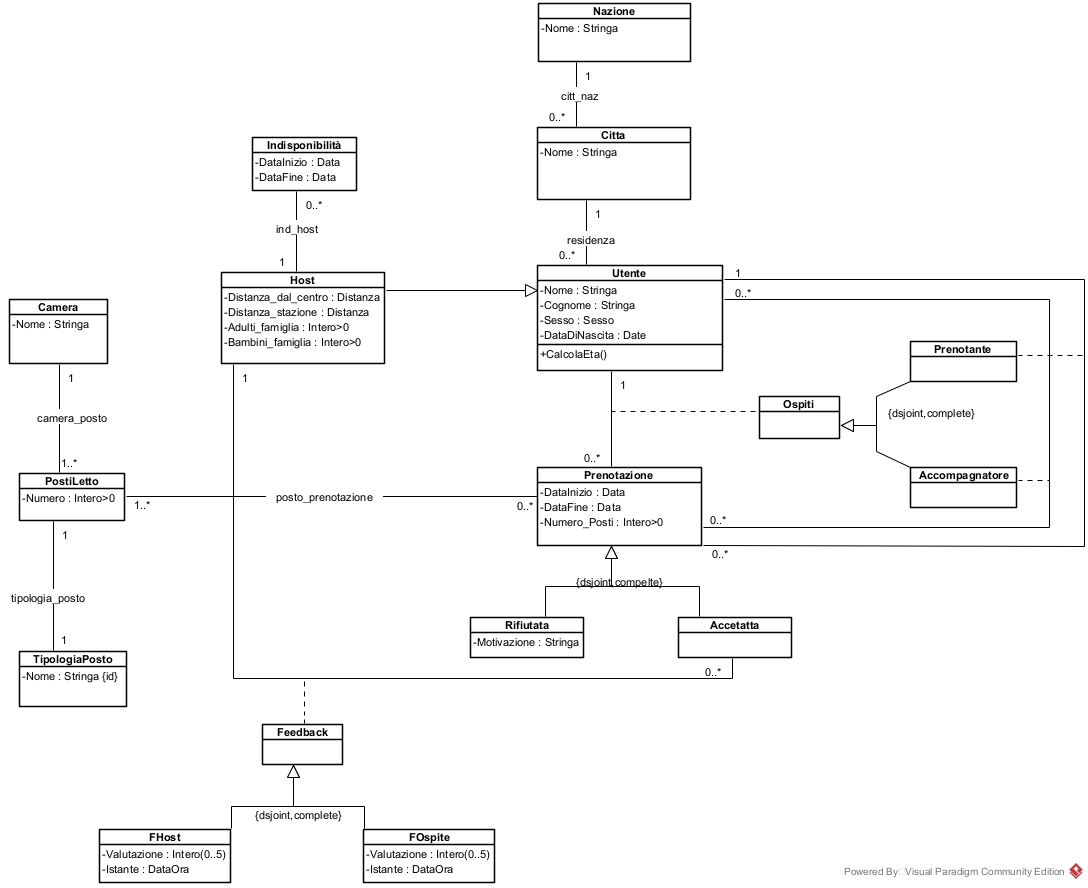
\includegraphics[width=1\textwidth ]{Images/UML.jpg}
\end{center} 
\newpage
\section{Tipi di Dato}
\begin{itemize}
    \item Distanza= $\{Km: Intero>0, m: Intero>0 \}$
    \item Sesso tipo enumerativo= $\{'Maschio', 'Femmina'\}$
\end{itemize}


\section{Vincoli Esterni}
I vincoli esterni del progetto sono:\\
\begin{itemize}
    \item $[V.Prenotazione.PrenotazioniPosto]$ \\
            Non possono esserci più prenotazioni dei posti letto per una camera.\\
    \item $[V.Feedback.HostObbligatorio]$\\
            Non può esistere una nuova prenotazione se l'utente prenotatore non ha lasciato un feedback all'host.\\
    \item $[V.Feedback.TerminePrenotazione]$\\
            Il feedback deve essere lasciato dopo il termine della prenotazione.\\
    \item $[V.Prenotazione.Indisponibilità]$\\
            Non si può effettuare una prenotazione se l'host è indisponibile.\\
\end{itemize}
\subsection{V.Prenotazione.PrenotazioniPosto}
$\forall p, pl,np,npl Prenotazione(p) \land PostiLetto(pl)\land PrenotazionePostoLetto(p,pl)$ \\ $\land NumeroPostiLetto(pl,npl) \land NumeroPostiPrenotazione(p,np)$ \\ \rightarrow $np \leq npl$
\subsection{V.Feedback.HostObbligatorio}
$\forall p, fp, fh, up Prenotazione(p) \land UtentePrenotante(p,up) \land FinePrenotazione(p,fp) \land adesso(a) \land a>fp \land FeedbackHostPrenotazione(p,fp)\land fp=Null $\\$\rightarrow \not \exists p2 Prenotazione(p2) \land UtentePrenotante(p2,up) \land p2!=p$
\subsection{V.Feedback.TerminePrenotazione}
\forall f, i, p, fp  \space $Prenotazione(p) \land FeedbackPrenotazione(f,p) \land IstanteFeedback(i,f)$\\ $\land FinePrenotazione(fp,p)$\\ $ \rightarrow fp <i$

\subsection{V.Prenotazione.Indisponibilità}
\forall h,ii,fi,p,ip, fp \space $ Host(h) \land InizioIndisponibilità(ii,h) \land FineIndisponibilità(fi,h)$\\ $\land Prenotazione(p) \land InizioPrenotazione(ip) \land FinePrenotazione(fp,p)$\\ $\rightarrow (ip<ii \land fp>ii) \lor (ip>fi \land fp>fi)$
\newpage
\section{Specifica Classi}

\section{Use-Case}
\subsection{Diagramma}
\begin{center}
    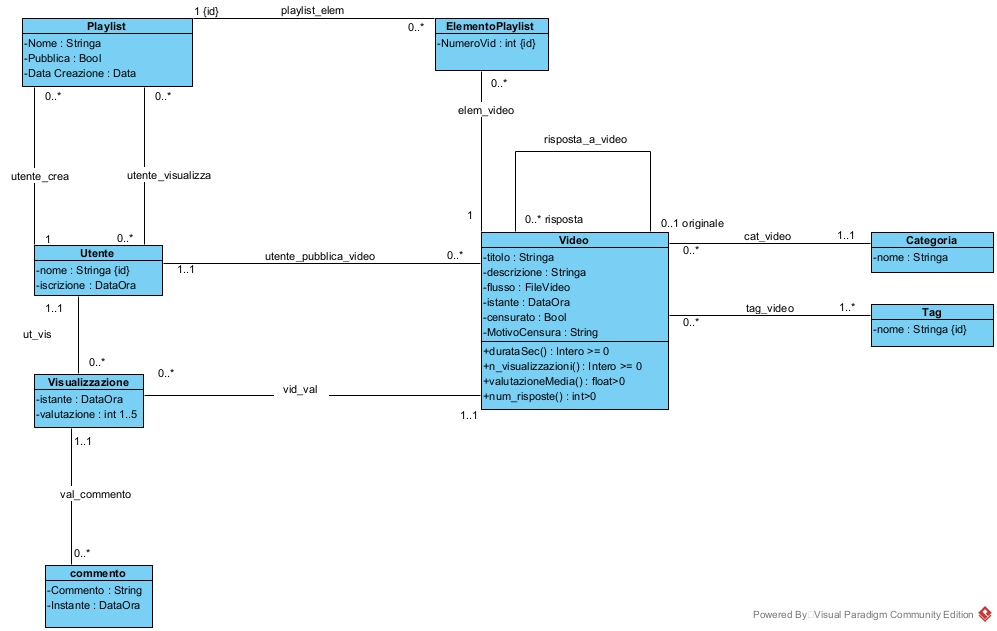
\includegraphics[width=1\textwidth ]{Images/UseCase.jpg}
\end{center} 
\newpage
\subsection{Specifica Use-Case}

    



\newpage
Arrivati a questo punto la fase di \textbf{Analisi} è \textbf{finita}.
\section{Ristrutturazione}
\subsection{Diagramma UML ristrutturato}
\begin{center}
    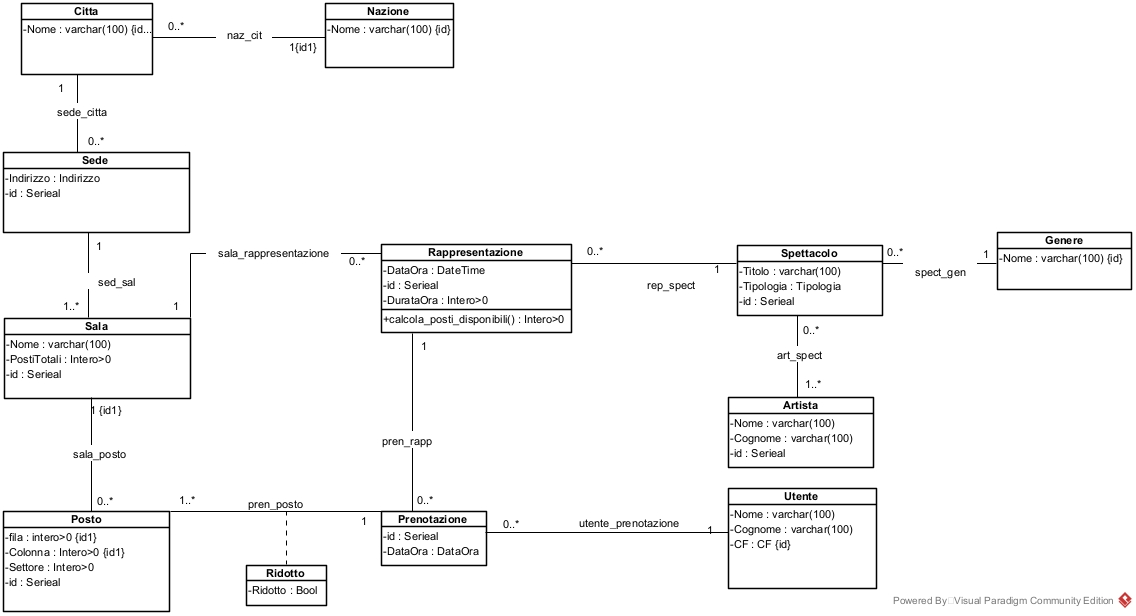
\includegraphics[width=1\textwidth ]{Images/UMLRistrutturato.jpg}
\end{center} 
\newpage
\textbf{Modifiche sulle generalizzazioni effettuate:}\\


\subsection{Tipi e Domini}
\subsubsection{Tipi}

\subsubsection{Domini}

\subsection{Vincoli Esterni}
Non sono stati inseriti nuovi vincoli esterni.
\subsection{Use Case}
Gli use case non violano la nuova ristrutturazione.
\newpage
\subsection{Traduzione diretta del diagramma UML delle classi ristrutturato}
Saranno scritte tutte le tabelle da creare:\\

\newpage \subsection{Trigger}
I vincoli esterni da controllare con i trigger sono:\\

\newpage \subsection{Progettazione Funzionalità}
Le Funzionalità da implementare nella base di dati sono:\\

\end{document}